\noindent
% ==================== CỘT LỀ TRÁI (HÌNH MINH HỌA) ====================
\begin{minipage}[t]{0.23\textwidth}
  \vspace{0pt}
  \centering
  % Hình cho Bài tập 4
  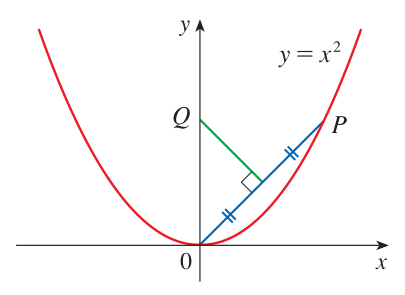
\includegraphics[width=\linewidth]{images/p0207_fig1.png}
  
  \vspace{5pt}
  {\fontsize{7.5pt}{9.5pt}\selectfont\textbf{\textsf{HÌNH CHO BÀI TẬP 4}}\par}

  % Khoảng cách dóng hàng chính xác tới Bài tập 10 theo bản đồ tọa độ gốc
  \vspace{166pt}

  % Hình cho Bài tập 10
  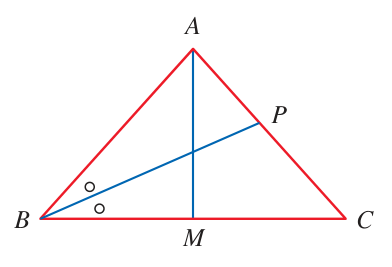
\includegraphics[width=\linewidth]{images/p0207_fig2.png}
  
  \vspace{5pt}
  {\fontsize{7.5pt}{9.5pt}\selectfont\textbf{\textsf{HÌNH CHO BÀI TẬP 10}}\par}
\end{minipage}%
\hfill
% ==================== CỘT CHÍNH (NỘI DUNG CÁC BÀI TẬP) ====================
\begin{minipage}[t]{0.73\textwidth}
  \vspace{0pt}
  \begin{enumerate}[label=\textbf{\arabic*.}, leftmargin=1.4em, itemsep=7pt, topsep=0pt, parsep=0pt]
    \setcounter{enumi}{3}

    % Bài tập 4
    \item Hình vẽ cho thấy một điểm $P$ trên parabol $y = x^2$ và điểm $Q$ là giao điểm của đường trung trực của đoạn $OP$ với trục $y$. Khi $P$ tiến dần về gốc tọa độ dọc theo parabol, điều gì sẽ xảy ra với $Q$? Điểm đó có vị trí giới hạn không? Nếu có, hãy tìm vị trí đó.

    % Bài tập 5
    \item Tính các giới hạn sau, nếu chúng tồn tại, trong đó $\llbracket x \rrbracket$ ký hiệu hàm phần nguyên lớn nhất.
    \vspace{2pt}
    
    \noindent
    \begin{tabular}{@{}p{0.48\linewidth}p{0.48\linewidth}@{}}
      \textbf{(a)} $\displaystyle \lim_{x \to 0} \frac{\llbracket x \rrbracket}{x}$ &
      \textbf{(b)} $\displaystyle \lim_{x \to 0} x \llbracket 1/x \rrbracket$
    \end{tabular}

    % Bài tập 6
    \item Phác thảo miền trong mặt phẳng được xác định bởi mỗi phương trình sau:
    \vspace{2pt}
    
    \noindent
    \begin{tabular}{@{}p{0.48\linewidth}p{0.48\linewidth}@{}}
      \textbf{(a)} $\llbracket x \rrbracket^2 + \llbracket y \rrbracket^2 = 1$ &
      \textbf{(b)} $\llbracket x \rrbracket^2 - \llbracket y \rrbracket^2 = 3$ \\[4pt]
      \textbf{(c)} $\llbracket x + y \rrbracket^2 = 1$ &
      \textbf{(d)} $\llbracket x \rrbracket + \llbracket y \rrbracket = 1$
    \end{tabular}

    % Bài tập 7
    \item Cho hàm số $f(x) = x/\llbracket x \rrbracket$.
    \vspace{2pt}
    
    \noindent
    \begin{tabular}{@{}p{0.48\linewidth}p{0.48\linewidth}@{}}
      \textbf{(a)} Tìm tập xác định và tập giá trị của $f$. &
      \textbf{(b)} Tính $\displaystyle \lim_{x \to -\infty} f(x)$.
    \end{tabular}

    % Bài tập 8
    \item Một \textbf{điểm bất động} của một hàm số $f$ là một số $c$ thuộc tập xác định của nó sao cho $f(c) = c$. (Hàm số không làm dịch chuyển $c$; nó vẫn giữ nguyên vị trí.)
    \begin{enumerate}[label=\textbf{(\alph*)}, leftmargin=1.5em, itemsep=2pt, topsep=2pt]
      \item Phác thảo đồ thị của một hàm số liên tục có tập xác định $[0, 1]$ mà tập giá trị cũng nằm trong $[0, 1]$. Xác định một điểm bất động của $f$.
      \item Hãy thử vẽ đồ thị của một hàm số liên tục có tập xác định $[0, 1]$ và tập giá trị nằm trong $[0, 1]$ mà \textit{không} có điểm bất động. Trở ngại ở đây là gì?
      \item Sử dụng Định lý Giá trị Trung gian để chứng minh rằng mọi hàm số liên tục có tập xác định $[0, 1]$ và tập giá trị nằm trong $[0, 1]$ đều phải có một điểm bất động.
    \end{enumerate}

    % Bài tập 9
    \item Nếu $\displaystyle \lim_{x \to a} [f(x) + g(x)] = 2$ và $\displaystyle \lim_{x \to a} [f(x) - g(x)] = 1$, hãy tìm $\displaystyle \lim_{x \to a} [f(x)g(x)]$.

    % Bài tập 10
    \item \textbf{(a)} Hình vẽ cho thấy một tam giác cân $ABC$ với $\angle B = \angle C$. Tia phân giác của góc $B$ cắt cạnh $AC$ tại điểm $P$. Giả sử cạnh đáy $BC$ được giữ cố định nhưng đường cao $|AM|$ của tam giác tiến dần về $0$, do đó $A$ tiến dần về trung điểm $M$ của $BC$. Điều gì xảy ra với $P$ trong quá trình này? Điểm đó có vị trí giới hạn không? Nếu có, hãy tìm vị trí đó.\\[3pt]
    \textbf{(b)} Hãy thử phác họa quỹ đạo được vạch ra bởi $P$ trong quá trình này. Sau đó tìm phương trình của đường cong này và dùng phương trình đó để phác họa đường cong.

    % Bài tập 11
    \item \textbf{(a)} Nếu xuất phát từ vĩ độ $0^\circ$ và đi theo hướng tây, ta có thể gọi $T(x)$ là nhiệt độ tại điểm $x$ ở bất kỳ thời điểm nào cho trước. Giả sử $T$ là một hàm liên tục của $x$, hãy chứng minh rằng tại một thời điểm cố định bất kỳ luôn tồn tại ít nhất hai điểm đối diện xuyên tâm trên đường xích đạo có cùng nhiệt độ chính xác.\\[3pt]
    \textbf{(b)} Kết quả ở phần (a) có còn đúng cho các điểm nằm trên một đường tròn bất kỳ trên bề mặt Trái Đất không?\\[3pt]
    \textbf{(c)} Kết quả ở phần (a) có đúng với áp suất khí quyển và với độ cao so với mực nước biển không?

    % Bài tập 12
    \item Nếu $f$ là hàm khả vi và $g(x) = x f(x)$, hãy dùng định nghĩa của đạo hàm để chứng minh rằng $g'(x) = x f'(x) + f(x)$.

    % Bài tập 13
    \item Giả sử $f$ là hàm số thỏa mãn phương trình
    \[
      f(x + y) = f(x) + f(y) + x^2 y + x y^2
    \]
    với mọi số thực $x$ và $y$. Giả sử thêm rằng
    \[
      \lim_{x \to 0} \frac{f(x)}{x} = 1
    \]
    \vspace{-2pt}
    \noindent
    \begin{tabular}{@{}p{0.3\linewidth}p{0.3\linewidth}p{0.35\linewidth}@{}}
      \textbf{(a)} Tìm $f(0)$. & \textbf{(b)} Tìm $f'(0)$. & \textbf{(c)} Tìm $f'(x)$.
    \end{tabular}

    % Bài tập 14
    \item Giả sử $f$ là hàm số có tính chất $|f(x)| \leqslant x^2$ với mọi $x$. Hãy chỉ ra rằng $f(0) = 0$. Sau đó hãy chứng minh rằng $f'(0) = 0$.
  \end{enumerate}
\end{minipage}

% ==================== CHÂN TRANG ====================
\vfill
\noindent
\begin{minipage}[b]{0.20\textwidth}
  {\fontsize{12pt}{14pt}\selectfont\textbf{\textsf{172}}}
\end{minipage}%
\hfill
\begin{minipage}[b]{0.77\textwidth}
  \fontsize{5.5pt}{6.8pt}\selectfont\color{copyrightgray}%
  Bản quyền thuộc Cengage Learning 2021. Mọi quyền được bảo lưu. Không được sao chép, quét hoặc nhân bản toàn bộ hay một phần. WCN 02-200-203\\
  Đánh giá biên tập đã xác nhận rằng nội dung bị ẩn không làm ảnh hưởng đáng kể đến trải nghiệm học tập tổng thể. Cengage Learning có quyền xóa nội dung bổ sung vào bất kỳ lúc nào nếu các hạn chế về quyền sau này yêu cầu.%
\end{minipage}
